\chapter{Psalm 37}

\begin{figure}
  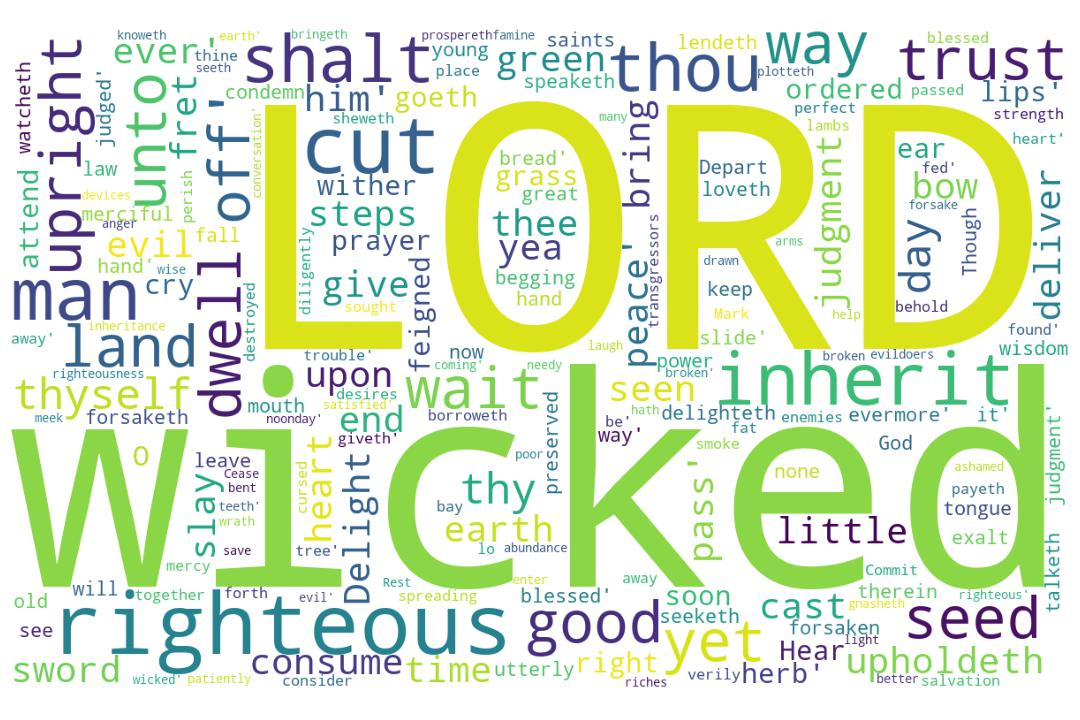
\includegraphics[width=\linewidth]{19OT-Psalms/Psalm37-WordCloud.jpg}
  \caption{Psalm 37 Word Cloud}
  \label{fig:Psalm 37  word Cloud}
\end{figure}

\marginpar{\scriptsize \centering \fcolorbox{bone}{lime}{\textbf{TEMPORARY TRIUMPH}}\\ (Psalm 37:1-40) \begin{compactenum}[I.][14]
   \item An \textbf{Apparent Problem} \index[scripture]{Psalms!Psa 037:01}(Psa 37:1) 
   \item An \textbf{Abundant Peace} \index[scripture]{Psalms!Psa 037:11}(Psa 37:11) 
   \item The \textbf{Aweful Potting} \index[scripture]{Psalms!Psa 037:12}(Psa 37:12) 
   \item The \textbf{Anticipated Perishing} \index[scripture]{Psalms!Psa 037:20}(Psa 37:20) 
    \item \textbf{Almighty Preservation} \index[scripture]{Psalms!Psa 037:28}(Psa 37:28)
    \item Their \textbf{Apparent Power} \index[scripture]{Psalms!Psa 037:35}(Psa 37:35)
    \item An \textbf{Awaited Passing} \index[scripture]{Psalms!Psa 037:36}(Psa 37:36)
    \item \textbf{Abandoned Paths} \index[scripture]{Psalms!Psa 037:01-11}(Psa 37:1--11)
    \item \textbf{Awesome Prophecies} \index[scripture]{Psalms!Psa 037:01-40}(Psa 37:1--40)
    \item \textbf{Attractive Pursuits} \index[scripture]{Psalms!Psa 037:11-22}(Psa 37:11--22)
    \item \textbf{Abiding Principles} \index[scripture]{Psalms!Psa 037:32-40}(Psa 37:32--40)
    \item \textbf{Absolute Promises} \index[scripture]{Psalms!Psa 037:01-11}(Psa 37:1--11)
\end{compactenum}}

\footnote{\textcolor[cmyk]{0.99998,1,0,0}{\hyperlink{TOC}{Return to end of Table of Contents.}}}\footnote{\href{https://audiobible.com/bible}{\textcolor[cmyk]{0.99998,1,0,0}{Psalm 37 Audio}}}\textcolor[cmyk]{0.99998,1,0,0}{\emph{A Psalm} of David.}\\
\\
\textcolor[cmyk]{0.99998,1,0,0}{Fret \fcolorbox{bone}{bone}{not} thyself because of \fcolorbox{bone}{lime}{evildoers}, neither be thou envious against the workers of iniquity.}
[2] \textcolor[cmyk]{0.99998,1,0,0}{For they shall soon be cut down like the grass, and wither as the green herb.}
[3] \textcolor[cmyk]{0.99998,1,0,0}{Trust in \fcolorbox{bone}{bone}{the LORD}, and do good; \emph{so} shalt thou dwell in the land, and verily thou shalt be fed.}
[4] \textcolor[cmyk]{0.99998,1,0,0}{Delight thyself also in \fcolorbox{bone}{bone}{the LORD}; and \fcolorbox{bone}{bone}{he} shall give thee the desires of thine heart.}
[5] \textcolor[cmyk]{0.99998,1,0,0}{Commit thy way unto \fcolorbox{bone}{bone}{the LORD}; trust also in him; and \fcolorbox{bone}{bone}{he} shall bring \emph{it} to pass.}
[6] \textcolor[cmyk]{0.99998,1,0,0}{And \fcolorbox{bone}{bone}{he} shall bring forth thy righteousness as the light, and thy judgment as the noonday.}
[7] \textcolor[cmyk]{0.99998,1,0,0}{Rest in \fcolorbox{bone}{bone}{the LORD}, and wait patiently for him: fret \fcolorbox{bone}{bone}{not} thyself because of him who prospereth in his way, because of the man who bringeth wicked devices to pass.}
[8] \textcolor[cmyk]{0.99998,1,0,0}{Cease from anger, and forsake wrath: fret \fcolorbox{bone}{bone}{not} thyself in any wise to do evil.}
[9] \textcolor[cmyk]{0.99998,1,0,0}{For evildoers shall be cut off: but those that wait upon \fcolorbox{bone}{bone}{the LORD}, they shall inherit the earth.}
[10] \textcolor[cmyk]{0.99998,1,0,0}{For yet a little while, and the wicked \emph{shall} \fcolorbox{bone}{bone}{not} \emph{be}: yea, thou shalt diligently consider his place, and it \emph{shall} \fcolorbox{bone}{bone}{not} \emph{be}.}
[11] \textcolor[cmyk]{0.99998,1,0,0}{But the meek shall inherit the earth; and shall delight themselves in the abundance of \fcolorbox{bone}{lime}{peace}.}\footnote{\textbf{Matthew 5;5} - Blessed are the meek: for they shall inherit the earth.}
[12] \textcolor[cmyk]{0.99998,1,0,0}{The wicked \fcolorbox{bone}{lime}{plotteth} against the just, and gnasheth upon him with his teeth.}
[13] \textcolor[cmyk]{0.99998,1,0,0}{The Lord shall laugh at him: for \fcolorbox{bone}{bone}{he} seeth that his day is coming.}
[14] \textcolor[cmyk]{0.99998,1,0,0}{The wicked have drawn out the sword, and have bent their bow, to cast down the poor and needy, \emph{and} to slay such as be of upright conversation.}
[15] \textcolor[cmyk]{0.99998,1,0,0}{Their sword shall enter into their own heart, and their bows shall be broken.}
[16] \textcolor[cmyk]{0.99998,1,0,0}{A little that a righteous man hath \emph{is} better than the riches of many wicked.}
[17] \textcolor[cmyk]{0.99998,1,0,0}{For the arms of the wicked shall be broken: but \fcolorbox{bone}{bone}{the LORD} upholdeth the righteous.}
[18] \textcolor[cmyk]{0.99998,1,0,0}{The LORD knoweth the days of the upright: and their inheritance shall be for ever.}
[19] \textcolor[cmyk]{0.99998,1,0,0}{They shall \fcolorbox{bone}{bone}{not} be ashamed in the evil time: and in the days of famine they shall be satisfied.}
[20] \textcolor[cmyk]{0.99998,1,0,0}{But the wicked shall \fcolorbox{bone}{lime}{perish}, and the enemies of \fcolorbox{bone}{bone}{the LORD} \emph{shall} \emph{be} as the fat of lambs: they shall consume; into smoke shall they consume away.}
[21] \textcolor[cmyk]{0.99998,1,0,0}{The wicked borroweth, and payeth \fcolorbox{bone}{bone}{not} again: but the righteous sheweth mercy, and giveth.}
[22] \textcolor[cmyk]{0.99998,1,0,0}{For \emph{such} \emph{as} \emph{be} blessed of him shall inherit the earth; and \emph{they} \emph{that} \emph{be} cursed of him shall be cut off.}
[23] \textcolor[cmyk]{0.99998,1,0,0}{The steps of a \emph{good} man are ordered by \fcolorbox{bone}{bone}{the LORD}: and \fcolorbox{bone}{bone}{he} delighteth in his way.}
[24] \textcolor[cmyk]{0.99998,1,0,0}{Though \fcolorbox{bone}{bone}{he} fall, \fcolorbox{bone}{bone}{he} shall \fcolorbox{bone}{bone}{not} be utterly cast down: for \fcolorbox{bone}{bone}{the LORD} upholdeth \emph{him} \emph{with} his hand.}
[25] \textcolor[cmyk]{0.99998,1,0,0}{I have been young, and \emph{now} am old; yet have I \fcolorbox{bone}{bone}{not} seen the righteous forsaken, nor his seed begging bread.}
[26] \textcolor[cmyk]{0.99998,1,0,0}{He \emph{is} ever merciful, and lendeth; and his seed \emph{is} blessed.}
[27] \textcolor[cmyk]{0.99998,1,0,0}{Depart from evil, and do good; and dwell for evermore.}
[28] \textcolor[cmyk]{0.99998,1,0,0}{For \fcolorbox{bone}{bone}{the LORD} loveth judgment, and forsaketh \fcolorbox{bone}{bone}{not} his saints; they are \fcolorbox{bone}{lime}{preserved} for ever: but the seed of the wicked shall be cut off.}
[29] \textcolor[cmyk]{0.99998,1,0,0}{The righteous shall inherit the land, and dwell therein for ever.}
[30] \textcolor[cmyk]{0.99998,1,0,0}{The mouth of the righteous speaketh wisdom, and his tongue talketh of judgment.}
[31] \textcolor[cmyk]{0.99998,1,0,0}{The law of his God \emph{is} in his heart; none of his steps shall slide.}
[32] \textcolor[cmyk]{0.99998,1,0,0}{The wicked watcheth the righteous, and seeketh to slay him.}
[33] \textcolor[cmyk]{0.99998,1,0,0}{The LORD will \fcolorbox{bone}{bone}{not} leave him in his hand, nor condemn him when \fcolorbox{bone}{bone}{he} is judged.}
[34] \textcolor[cmyk]{0.99998,1,0,0}{Wait on \fcolorbox{bone}{bone}{the LORD}, and keep his way, and \fcolorbox{bone}{bone}{he} shall exalt thee to inherit the land: when the wicked are cut off, thou shalt see \emph{it}.}
[35] \textcolor[cmyk]{0.99998,1,0,0}{I have seen the wicked in great \fcolorbox{bone}{lime}{power}, and spreading himself like a green bay tree.}\footnote{\textbf{Matthew 13:31-32} - Another parable put he forth unto them, saying, The kingdom of heaven is like to a grain of mustard seed, which a man took, and sowed in his field: [32 ]Which indeed is the least of all seeds: but when it is grown, it is the greatest among herbs, and becometh a tree, so that the birds of the air come and lodge in the branches thereof.}
[36] \textcolor[cmyk]{0.99998,1,0,0}{Yet \fcolorbox{bone}{bone}{he} \fcolorbox{bone}{lime}{passed} away, and, lo, \fcolorbox{bone}{bone}{he} \emph{was} \fcolorbox{bone}{bone}{not}: yea, I sought him, but \fcolorbox{bone}{bone}{he} could \fcolorbox{bone}{bone}{not} be found.}
[37] \textcolor[cmyk]{0.99998,1,0,0}{Mark the perfect \emph{man}, and behold the upright: for the end of \emph{that} man \emph{is} peace.}
[38] \textcolor[cmyk]{0.99998,1,0,0}{But the transgressors shall be destroyed together: the end of the wicked shall be cut off.}
[39] \textcolor[cmyk]{0.99998,1,0,0}{But the salvation of the righteous \emph{is} of \fcolorbox{bone}{bone}{the LORD}: \emph{he} \emph{is} their strength in the time of trouble.}\footnote{\textbf{Job 38:23} - Which I have reserved against the time of trouble, against the day of battle and war?}\footnote{\textbf{Psalm 27:15} - For in the time of trouble he shall hide me in his pavilion: in the secret of his tabernacle shall he hide me; he shall set me up upon a rock.}\footnote{\textbf{Psalm 41:1} - Blessed is he that considereth the poor: the LORD will deliver him in time of trouble.}\footnote{\textbf{Proverb 25:19} - Confidence in an unfaithful man in time of trouble is like a broken tooth, and a foot out of joint.}\footnote{\textbf{Isaiah 33:2} -O LORD, be gracious unto us; we have waited for thee: be thou their arm every morning, our salvation also in the time of trouble.}\footnote{\textbf{Jeremiah 14:18} - O the hope of Israel, the saviour thereof in time of trouble, why shouldest thou be as a stranger in the land, and as a wayfaring man that turneth aside to tarry for a night?}\footnote{\textbf{Daniel 12:1} - And at that time shall Michael stand up, the great prince which standeth for the children of thy people: and there shall be a time of trouble, such as never was since there was a nation even to that same time: and at that time thy people shall be delivered, every one that shall be found written in the book.}
[40] \textcolor[cmyk]{0.99998,1,0,0}{And \fcolorbox{bone}{bone}{the LORD} shall help them, and deliver them: \fcolorbox{bone}{bone}{he} shall deliver them from the wicked, and save them, because they trust in him.}



